\documentclass[a4paper,12pt]{article}

\title{Chapter 2. The Klein-Gordon Field\\
2-1. The necessary of the Field Viewpoint}
\date{各種SNS\\
    X (旧 Twitter): \href{https://x.com/miya_max_study}{@miya\_max\_study}\\
    Instagram : \href{https://www.instagram.com/daily_life_of_miya/}{@daily\_life\_of\_miya}\\
    YouTube : \href{https://www.youtube.com/@miya-max-active}{@miya-max-active}
    }
\author{Max Miyazaki}

\usepackage{amsmath}
\usepackage{amssymb}
\usepackage{ascmac}
\usepackage{amsthm}
\usepackage{amsfonts}
\usepackage{enumitem}
\usepackage{color}
\usepackage[dvipdfmx]{graphicx}
\usepackage{float}
\usepackage{bm}
\usepackage{here}

\usepackage{abstract}
\usepackage{tikz}
\usetikzlibrary{shapes.geometric, arrows.meta, positioning}
\usepackage{indentfirst}
\usepackage[utf8]{inputenc}
\usepackage{fix-cm}
\usepackage{wrapfig}
\pagenumbering{arabic}
\usepackage{url}
\usepackage{xcolor}
\usepackage[most]{tcolorbox}
\usepackage{framed}
\usepackage[dvipdfmx]{hyperref}
\hypersetup{
 setpagesize=false,
 bookmarksnumbered=true,
 colorlinks=true,
 linkcolor=blue
}

% Define braket-like commands
\newcommand{\bra}[1]{\left\langle #1\right|}
\newcommand{\ket}[1]{\left|#1\right\rangle}
\newcommand{\braket}[2]{\left\langle #1\middle|#2\right\rangle}
\newcommand{\brakets}[3]{\left\langle #1\middle| #2 \middle|#3 \right\rangle}

\renewcommand{\arraystretch}{2.1}


\setlength{\textwidth}{16cm}
\setlength{\textheight}{25cm}
\setlength{\oddsidemargin}{0cm}
\setlength{\evensidemargin}{0cm}
\setlength{\topmargin}{-2cm}

\begin{document}
\maketitle

\vspace{1cm}
\begin{abstract}
    このノートはPeskin\&Schroederの``An Introduction to Quantum Field Theory''の第2章の1節をまとめたものである. 要点や個人的な追記, 計算ノート的なまとめを行っているが, それらはすべて原書の内容を出発点としている. 参考程度に使っていただきたいが, このノートは私の勉強ノートであり, そのままの内容をそのまま鵜呑みにすると間違った理解を招く可能性があることをご了承ください. ぜひ原著を手に取り, その内容をご自身で確認していただくことを推奨します. てへぺろ v$({\hat{\cdot}_\partial \hat{\cdot}})$v



\end{abstract}
    
    

\newpage
\section*{2.1 The necessary of the Field Viewpoint}

\begin{itemize}
    \item \textbf{場の量子論とは} \\
    量子力学が粒子の力学系を量子化するように, 場の量子論は場の力学系に量子力学を適用したものである. \par
    \textcolor{blue}{※簡単のためにそう説明されているが, 実際には局所性と特殊相対性理論も考える必要があるので, 以下のように理解しておくと良い. 
    \begin{center}
        場の量子論 = 局所性 + 特殊相対性理論 + 量子力学
    \end{center}}
  
    \item \textbf{素粒子論における重要性} \\
    素粒子論の現状を理解するには場の量子論が欠かせない. \\
    本書の第1部では主に相対論的な場(素粒子)について議論する.\par
    \textcolor{blue}{※みなさんも一緒に頑張りましょう!}
  
    \item \textbf{他分野への応用可能性} \\
    原子物理学, 核物理学, 凝縮系物理学などにも応用可能であり, 多少の修正を加えることで重要な役割を果たす.
  
    \item \textbf{読者の疑問} \\
    極小(量子力学的)スケールと極大(相対論的)スケールの現象を理解するために, なぜ場の量子化が必要なのかと疑問に思う読者もいるのでは?
  
    \item \textbf{相対論的粒子を単純に量子化できないのか?} \\
    非相対論的な粒子と同様に, 相対論的粒子も1粒子理論で量子化できるのではないかという疑問が生じる.
  
    \item \textbf{例:波動関数による検討} \\
    Klein-Gordon方程式やDirac方程式により1粒子の相対論的波動関数を書き下し, 負エネルギー状態や不合理が現れるかを検討する方法がある.
  
    \item \textbf{ここでは議論を省略} \\
    この議論は多くの量子力学の教科書に委ね, 本文では詳細に立ち入らない.
  
    \item \textbf{簡単な理解:対生成の観点} \\
    Einsteinの関係 $E = mc^2$ は粒子と反粒子の対生成が起こり得ることを意味しており, 1粒子理論では相対論的過程を説明できない.
  
    \item \textbf{エネルギーが不十分な場合でも多粒子状態は現れる} \\
    たとえば2次の摂動論における中間状態などにおいて多粒子状態が現れる.
  
    \item \textbf{高次摂動論での仮想粒子の登場} \\
    摂動論を高次まで進めると, 中間状態に現れる「仮想」粒子は多く生成される.
\end{itemize}
  
多粒子理論の必要性は, 因果律を考慮した非自明な場合にも現れる. 自由粒子が点 $\boldsymbol{x}_0$ から点 $\boldsymbol{x}$ まで伝播する確率振幅 $U(t)$ を考えてみる:

\begin{equation*}
  U(t) = \langle \boldsymbol{x} | e^{-iHt} | \boldsymbol{x}_0 \rangle.
\end{equation*}
  
非相対論的量子力学において, 粒子のエネルギー $E$ は運動量 $\boldsymbol{p}$ を用いて $E = \boldsymbol{p}^2 / 2m$ と書けるので, 上式は次のようになる.
  
\begin{align*}
  U(t) &= \langle \boldsymbol{x} | e^{-i(\boldsymbol{p}^2 / 2m)t} | \boldsymbol{x}_0 \rangle \\
  &= \int d^3 p \, \langle \boldsymbol{x} | e^{-i(\boldsymbol{p}^2 / 2m)t} | \boldsymbol{p} \rangle \langle \boldsymbol{p} | \boldsymbol{x}_0 \rangle \\
  &= \frac{1}{(2\pi)^3} \int d^3p \, e^{-i(\boldsymbol{p}^2 / 2m)t} \cdot e^{i\boldsymbol{p} \cdot (\boldsymbol{x} - \boldsymbol{x}_0)} \\
  &= \left( \frac{m}{2\pi i t} \right)^{3/2} e^{im(\boldsymbol{x} - \boldsymbol{x}_0)^2 / 2t}.
\end{align*}
  
\color{blue}
\begin{proof}

※上の計算を確認する.\\

\begin{equation*}\label{2.a1}
  U(t) = \langle \boldsymbol{x} | e^{-i(\boldsymbol{p}^2 / 2m)t} | \boldsymbol{x}_0 \rangle \tag{2-1.a1}
\end{equation*}

について運動量固有状態の完全性関係

\begin{equation*}
    \int d^3p\, |\boldsymbol{p} \rangle \langle \boldsymbol{p}| = \mathbf{1} \tag{2-1.a2}
\end{equation*}

を代入すると, 

\begin{equation*}
    U(t) = \int d^3p\, \langle \boldsymbol{x} | e^{-i(\boldsymbol{p}^2 / 2m)t} | \boldsymbol{p} \rangle \langle \boldsymbol{p} | \boldsymbol{x}_0 \rangle \tag{2-1.a3}
\end{equation*}

となる. ここで, ブラケットの計算は量子力学の内容を思い出すと, 

\begin{equation*}
    \langle \boldsymbol{x} | \boldsymbol{p} \rangle = \frac{1}{(2\pi)^{3/2}} e^{i \boldsymbol{p} \cdot \boldsymbol{x}}, \quad \langle \boldsymbol{p} | \boldsymbol{x}_0 \rangle = \frac{1}{(2\pi)^{3/2}} e^{-i \boldsymbol{p} \cdot \boldsymbol{x}_0} \tag{2-1.a4}
\end{equation*}

となるので (ここまでの議論が分からない人はこちらを参照),

\begin{align*}\label{2.a5}
    U(t) &= \frac{1}{(2\pi)^3} \int d^3p \, e^{-i(\boldsymbol{p}^2 / 2m)t} \cdot e^{i\boldsymbol{p} \cdot (\boldsymbol{x} - \boldsymbol{x}_0)} \tag{2-1.a5}
\end{align*} 

となる. これは $3$ 次元の Fourier 積分であり, Gaussian 積分として評価できる.

\begin{align*}
    U(t) &= \left( \frac{m}{2\pi i t} \right)^{3/2} e^{i m (\boldsymbol{x} - \boldsymbol{x}_0)^2 / 2t}. \tag{2-1.a6}
\end{align*}

この積分を評価してみよう. 見やすさのために指数関数は $\exp[x]$ 表示にしている:

\begin{equation*}
U(t) = \frac{1}{(2\pi)^3} \int d^3p \, \exp\left[ -i \frac{\boldsymbol{p}^2}{2m} t + i \boldsymbol{p} \cdot (\boldsymbol{x} - \boldsymbol{x}_0) \right]. \tag{2-1.a7}
\end{equation*}

ここで, \(\boldsymbol{r} = \boldsymbol{x} - \boldsymbol{x}_0\) と置くと, 積分は次のようになる:

\begin{equation*}
U(t) = \frac{1}{(2\pi)^3} \int d^3p \, \exp\left[ -i \frac{\boldsymbol{p}^2}{2m} t + i \boldsymbol{p} \cdot \boldsymbol{r} \right]. \tag{2-1.a8}
\end{equation*}

この積分は, 3次元の Gaussian 型積分なので, 成分ごとに分けて評価できる:

\begin{equation*}
U(t) = \left( \frac{1}{2\pi} \right)^3 \prod_{j = 1}^3 \int_{-\infty}^{\infty} dp_j \, \exp\left[ -i \frac{p_j^2}{2m} t + i p_j r_j \right]. \tag{2-1.a9}
\end{equation*}

各方向の積分は Gaussian 積分の変形であり, 次の公式を使う:

\begin{equation*}
\int_{-\infty}^\infty dp \, \exp\left( -a p^2 + b p \right) = \sqrt{ \frac{\pi}{a} } \exp\left( \frac{b^2}{4a} \right),
\quad \text{Re}(a) > 0. \tag{2-1.a10}
\end{equation*}

今回の積分では \( a = i \frac{t}{2m} \), \( b = i r_j \), よって

\begin{equation*}
\int_{-\infty}^{\infty} dp_j \, \exp\left[ -i \frac{p_j^2}{2m} t + i p_j r_j \right]
= \sqrt{ \frac{2\pi m}{i t} } \exp\left( i \frac{m r_j^2}{2t} \right). \tag{2-1.a11}
\end{equation*}

これを3方向分かけ合わせると:

\begin{align*}
U(t) &= \left( \frac{1}{2\pi} \right)^3 \left( \frac{2\pi m}{i t} \right)^{3/2}
\exp\left( i \frac{m}{2t} \sum_{j=1}^3 r_j^2 \right) \\
&= \left( \frac{m}{2\pi i t} \right)^{3/2} \exp\left( i \frac{m (\boldsymbol{x} - \boldsymbol{x}_0)^2}{2t} \right). \tag{2-1.a12}
\end{align*}
\end{proof}


\color{black}
この式は任意の $x = \| \boldsymbol{x} - \boldsymbol{x}_0 \|$ と $t$ に対して non-zero なので, 粒子は任意の2点間をいくらでも短い時間で移動できることになる. 相対論的理論では, この結果は因果律の破れを意味する. 従って相対論的表式 $E = \sqrt{\boldsymbol{p}^2 + m^2}$ を用いれば解決できるように思えるが, そうもいかない.\par
\textcolor{blue}{※因果律の破れが起きてしまったのは, エネルギーの表示で非相対論的なエネルギー $E = \boldsymbol{p}^2/2m$ を用いたのが原因かもしれない. なので相対論的に正しいエネルギーの表示 $E = \sqrt{\boldsymbol{p}^2 + m^2}$ を使えば解決するだろうという思惑を持って因果律を破らないか計算してみると, 実はこれもうまくいかないことが次の議論により分かる.} \\
この表式を用いて同じ計算をすると, 球座標 $(p, \theta, \varphi)$ への変数変換により以下を得る.

\begin{align*}
  U(t) &= \langle \boldsymbol{x} | e^{-it\sqrt{\boldsymbol{p}^2 + m^2}} | \boldsymbol{x}_0 \rangle \\
  &= \frac{1}{(2\pi)^3} \int d^3p \, e^{-it\sqrt{\boldsymbol{p}^2 + m^2}} \cdot e^{i\boldsymbol{p} \cdot (\boldsymbol{x} - \boldsymbol{x}_0)} \\
  &= \frac{1}{2\pi^2 \| \boldsymbol{x} - \boldsymbol{x}_0 \|} \int_0^\infty dp \, p \sin(p \| \boldsymbol{x} - \boldsymbol{x}_0 \|) e^{-it\sqrt{p^2 + m^2}}
\end{align*}

\color{blue}
\begin{proof} ※上の計算を確認する.

\begin{align*}
  U(t) &= \langle \boldsymbol{x} | e^{-it\sqrt{\boldsymbol{p}^2 + m^2}} | \boldsymbol{x}_0 \rangle \tag{2-1.b1} \\
      &= \frac{1}{(2\pi)^3} \int d^3p \, e^{-it\sqrt{\boldsymbol{p}^2 + m^2}} \cdot e^{i\boldsymbol{p} \cdot (\boldsymbol{x} - \boldsymbol{x}_0)}. \tag{2-1.b2}
\end{align*}
これは \eqref{2.a1} から \eqref{2.a5} と同じ計算なので省略. \\
3次元運動量空間の積分を球座標に変換すると,球座標内では次のようになる.

\begin{align*}
  \boldsymbol{p} &= (p, \theta, \varphi), \tag{2-1.b3}\\
  d^3p &= p^2 \sin \theta \, dp \, d\theta \, d\varphi, \tag{2-1.b4}\\
  \boldsymbol{p} \cdot (\boldsymbol{x} - \boldsymbol{x}_0) &= p \| \boldsymbol{x} - \boldsymbol{x}_0 \| \cos \theta. \label{2.b3}\tag{2-1.b5}
\end{align*}

\begin{framed}
※余談\\
\eqref{2.b3} の内積について, 少しトリックを使っている. ここで $\theta$ は $p$ と $\boldsymbol{x} - \boldsymbol{x}_0$ のなす角だと勝手に決めている. なぜなら, もし一般的にベクトル $\boldsymbol{r} = \boldsymbol{x} - \boldsymbol{x}_0$ が任意の向きを向いていた場合, ベクトル $\boldsymbol{p}$ となす角 $\theta_{\textrm{pr}}$ は球座標の $\theta$ と一致せず, 例えば $\cos\theta_{\textrm{pr}} = \sin\theta \sin\theta_r \cos(\varphi - \varphi_r) + \cos\theta\cos\theta_r$ (一般に2つのベクトルのなす角の公式) のような複雑な三角関数の組み合わせが現れてしまう. つまり, $\eqref{2.b6}$ の $\theta$, $\varphi$ 積分が複雑になってしまう. そこで $\boldsymbol{p}$ の $z$ 軸を回転させて $\boldsymbol{r} = \boldsymbol{x} - \boldsymbol{x}_0$ の方向に合わせると, 球座標で定義される $\theta$ と $\boldsymbol{p}$, $\boldsymbol{r}$ がなす角 $\theta_r$ が一致して単純な $\cos\theta$ が積分の中に現れるだけで済む. 勝手にこのような操作をして大丈夫か不安になる方もいるだろうが, 運動量空間の積分は全範囲で行なっているので, 座標系の回転は結果に影響を与えないので大丈夫. 物理学ではこのような対称性 (今回は回転対称性) を利用して, 計算を楽にするという手段は非常に使う考え方の一つなので押さえておくと良いだろう. 
\end{framed}

\noindent よって, 積分は次のように変換される:

\begin{align*}\label{2.b6}
  U(t) &= \frac{1}{(2\pi)^3} \int_0^\infty dp \, \int_{0}^{\pi} d\theta \, \int_{0}^{2\pi} d\varphi \, p^2 \sin \theta \, e^{-it\sqrt{p^2 + m^2}} \cdot e^{i p \| \boldsymbol{x} - \boldsymbol{x}_0 \| \cos \theta}. \tag{2-1.b6}
\end{align*}
$\varphi$ については積分が

\begin{equation*}
  \int_{0}^{2\pi} d\varphi = 2\pi, \tag{2-1.b7}
\end{equation*} 
と自明だが, $\theta$ 積分については少々計算が面倒であるので確認しておく.

\begin{equation*}
  \int_{0}^{\pi} d\theta \, \sin \theta \, e^{i p \| \boldsymbol{x} - \boldsymbol{x}_0 \| \cos \theta}. \tag{2-1.b8}
\end{equation*}
この $\theta$ 積分について, $r = \| \boldsymbol{x} - \boldsymbol{x}_0 \|$ と置くと, 

\begin{equation*}
  \int_{0}^{\pi} d\theta \, \sin \theta \, e^{i p r \cos \theta}. \tag{2-1.b9}
\end{equation*}
ここで $u = \cos \theta$ と変数変換をすると, $du = -\sin \theta d\theta$, $0 \leq \theta \leq \pi \to -1 \leq u \leq 1$ より, 

\begin{align*}
  \int_{0}^{\pi} d\theta \, \sin \theta \, e^{i p r \cos \theta} &= \int_{-1}^{1} du \, e^{i p r u} \tag{2-1.b10}\\
  &= \left[\frac{e^{i p r u}}{i p r}\right]_{-1}^{1} \tag{2-1.b11} \\
  &= \frac{e^{i p r} - e^{-i p r}}{i p r} \tag{2-1.b12} \\
  &= \frac{2\sin(p r)}{p r}. \tag{2-1.b13}
\end{align*}
したがって, \eqref{2.b6} は次のようになる:

\begin{align*}
  U(t) &= \frac{1}{(2\pi)^3} \int_0^\infty dp \, \int_{0}^{\pi} d\theta \, \int_{0}^{2\pi} d\varphi \, p^2 \sin \theta \, e^{-it\sqrt{p^2 + m^2}} \cdot e^{i p \| \boldsymbol{x} - \boldsymbol{x}_0 \| \cos \theta} \tag{2-1.b14} \\
  &= \frac{1}{(2\pi)^3} \, 2\pi \int_0^\infty dp \, p^2 \cdot \frac{2\sin(p r)}{p r} \cdot e^{-it\sqrt{p^2 + m^2}} \tag{2-1.b15}\\
  &= \frac{1}{2\pi^2 r} \int_0^\infty dp \, p\sin(p r)\cdot e^{-it\sqrt{p^2 + m^2}} \tag{2-1.b16}\\
  &= \frac{1}{2\pi^2 \| \boldsymbol{x} - \boldsymbol{x}_0 \|} \int_0^\infty dp \, p \sin(p \| \boldsymbol{x} - \boldsymbol{x}_0 \|) e^{-it\sqrt{p^2 + m^2}}. \tag{2-1.b17}
\end{align*}


\end{proof}

\color{black}

  
この積分はBessel関数を用いて表せるが \textcolor{blue}{(※僕の理解不足なため, 実際に Bessel 関数を用いた計算はパスします\dots)}, ここでは停留位相近似によって光円錐の外側遠方, 即ち $x^2 \gg t^2$ に於ける漸近的な振舞いを見ることにしよう. 指数関数の引数 $px - t\sqrt{p^2 + m^2}$ の定数倍を $\phi(p)$ とすれば, この関数は $p = imx / \sqrt{x^2 - t^2}$ に停留点を持つ. 従ってこの点を通るように積分経路を自由に動かすことができ, 停留点の表式を上式の $p$ に代入すれば, 確率振幅 $U(t)$ は $x$ と $t$ の有理関数をかけた形で
  
\begin{equation*}
  U(t) \sim e^{-m\sqrt{x^2 - t^2}}
\end{equation*}
  
という形になることが分かる.\par
\color{blue}
この積分の評価方法を停留位相法といい, 振動積分 $\displaystyle \int_{-\infty}^{\infty} dp \, e^{i\lambda \phi(p)a(p)}$ のような形に対して, $\lambda \to \infty$ のときに,
\begin{itemize}
  \item 位相 $\phi(p)$ の導関数がゼロになる点 (停留点) 付近が支配的になる.
  \item 他の場所では位相が早く振動して積分値が小さくなる (指数関数的に減衰する).
\end{itemize}
という性質がある. これを利用して, 積分を漸近的に評価する方法を停留位相法という.
\vskip\baselineskip
\color{blue}
\begin{proof} ※確率振幅 $U(t)$ が $x$ と $t$ の有理関数になることを示す.\\
目標:$x^2 \gg t^2$ の領域 (光円錐の外側) で次の積分の漸近的振る舞いを見る.

\begin{equation*}
  U(t) = \frac{1}{2\pi^2 \| \boldsymbol{x} - \boldsymbol{x}_0 \|} \int_0^\infty dp \, p \sin(p \| \boldsymbol{x} - \boldsymbol{x}_0 \|) e^{-it\sqrt{p^2 + m^2}}. \tag{2-1.c1}
\end{equation*}

$r = \| \boldsymbol{x} - \boldsymbol{x}_0 \|$ と置くと, 

\begin{equation*}\label{2.c2}
  U(t) = \frac{1}{2\pi^2 r} \int_0^\infty dp \, p \sin(p r) e^{-it\sqrt{p^2 + m^2}}. \tag{2-1.c2}
\end{equation*}

$\sin(p r) = \dfrac{e^{ipr} - e^{-ipr}}{2i}$ より, \eqref{2.c2} は次のように計算される.

\begin{align*}
  U(t) &= \frac{1}{2\pi^2 r} \int_0^\infty dp \, p \left( \frac{e^{ipr} - e^{-ipr}}{2i} \right) e^{-it\sqrt{p^2 + m^2}} \tag{2-1.c3}\\
  &= \frac{1}{4\pi^2 ir} \int_0^\infty dp \, p \left( e^{ipr} - e^{-ipr} \right) e^{-it\sqrt{p^2 + m^2}} \tag{2-1.c4} \\
  &= \frac{1}{4\pi^2 ir} \int_0^\infty dp \, p \left( \exp\left[i(pr - t\sqrt{p^2 + m^2})\right] - \exp\left[-i(pr - t\sqrt{p^2 + m^2})\right] \right). \label{2-1.c5}\tag{2-1.c5}
\end{align*}

ここで括弧の2つの項をそれぞれ

\begin{align*}
  I_+ &= \int_0^\infty dp \, p \exp\left[i(pr - t\sqrt{p^2 + m^2})\right] \tag{2-1.c6} \\
  I_- &= \int_0^\infty dp \, p \exp\left[-i(pr - t\sqrt{p^2 + m^2})\right] \tag{2-1.c7}
\end{align*}

とおくと, $I_+$ の複素共役が $I_-$ なので,

\begin{equation*}
  I_+(t) - I_-(t) = I_+(t) - (I_+(t))^* = 2i \, \textrm{Im}\, I_+(t). \tag{2-1.c8}
\end{equation*}

よって, \eqref{2.c5} は次のように計算される.

\begin{align*}
  U(t) &= \frac{1}{4\pi^2 ir} \left( I_+(t) - I_-(t) \right) \tag{2-1.c9} \\
  &= \frac{1}{4\pi^2 ir} \left( 2i \, \textrm{Im}\, I_+(t) \right) \tag{2-1.c10} \\
  &= \frac{1}{2\pi^2 r} \, \textrm{Im}\, I_+(t). \tag{2-1.c11}
\end{align*}

これにより, 確率振幅 $U(t)$ の解析では $I_+(t)$ だけ解析すれば良いことが分かる.\par
指数関数の位相の引数を次のように定義する:

\begin{equation*}
  \phi(p) = pr - t\sqrt{p^2 + m^2}. \tag{2-1.c12}
\end{equation*}

この関数の停留点 $\dfrac{d\phi}{dp} = 0$ は,

\begin{equation*}
  \frac{d\phi}{dp} = r - \frac{tp}{\sqrt{p^2 + m^2}} = 0 \tag{2-1.c13}
\end{equation*}
\begin{align*}
  \frac{tp}{\sqrt{p^2 + m^2}} &= r \tag{2-1.c14} \\
  \frac{p}{\sqrt{p^2 + m^2}} &= \frac{r}{t} \tag{2-1.c15} \\
  \frac{p^2}{p^2 + m^2} &= \frac{r^2}{t^2} \to p^2 = -\frac{m^2 r^2}{r^2t^2 - m^2} \tag{2-1.c16}
\end{align*}

したがって, 停留点 $p_s$ は

\begin{equation*}
  p_s = \frac{imr}{\sqrt{r^2 - t^2}}, \hspace{0.5cm} (r^2 \gg t^2). \tag{2-1.c17}
\end{equation*}

停留点 $p_s$ が虚数軸上 ($r^2 \gg t^2$, space-like な距離) にあるとき, 積分経路を複素平面に沿って変形することができる. この点を通るように積分経路を自由に動かすことができる.\\
Cauchy の定理から解析関数 $f(p)$ に対して, 閉曲線上 $\Gamma$ の積分はゼロ,

\begin{equation*}
  \int_\Gamma dp \, f(p) = 0. \tag{2-1.c18}
\end{equation*}

つまり, 積分経路を複素平面に沿って変形しても, 被積分関数が解析的 (特異点を持たない) ならば積分値は変わらない. 今回のケースでは, 被積分関数 $f(p) = p \exp\left[i(pr - t\sqrt{p^2 + m^2})\right]$ は $p \in \mathbb{C}$ で branch cut (分岐線) を避ければ解析的である. 物理的に都合の良い branch cut の取り方は $[im, \infty)$ と $(-\infty, -im]$ の2本の直線である. branch point は $p = \pm im$ で 停留点 $p_s = imr/\sqrt{r^2 - t^2}$ はこの2本の直線の間にあるため特異点を含まないので Cauchy の定理が適用できる. 
\vskip\baselineskip
積分の主な寄与は停留点近傍からくるので, 積分全体は以下のように近似できる:

\begin{equation*}\label{2-1.c19}
  U(t) \sim A(r,t) \cdot \exp\left[i(p_s r - t\sqrt{p_s^2 + m^2})\right] \tag{2-1.c19}
\end{equation*}

ここで $A(r,t)$ は振幅の前にかかるゆっくりと変化する係数 (有理関数) である.\par
$p_s r = imr^2/\sqrt{r^2 - t^2}$, $p_s^2 = -m^2 r^2/(r^2 - t^2)$ より, \eqref{2-1.c19} は次のように計算される:

\begin{align*}
  U(t) &\sim A(r,t) \cdot \exp\left[i\left( \frac{imr^2}{\sqrt{r^2 - t^2}} - t \sqrt{-\frac{m^2 r^2}{r^2 - t^2} + m^2} \right)\right] \tag{2-1.c21} \\
  &= A(r,t) \cdot \exp\left[i\left( \frac{imr^2}{\sqrt{r^2 - t^2}} - mt \sqrt{-\frac{ r^2}{r^2 - t^2} + 1} \right)\right] \tag{2-1.c22}\\
  &= A(r,t) \cdot \exp\left[i\left( \frac{imr^2}{\sqrt{r^2 - t^2}} - mt \sqrt{-\frac{ r^2}{r^2 - t^2} + \frac{r^2 - t^2}{r^2 - t^2}} \right)\right] \tag{2-1.c23}\\
  &= A(r,t) \cdot \exp\left[i\left( \frac{imr^2}{\sqrt{r^2 - t^2}} - mt \sqrt{\frac{-t^2}{r^2 - t^2}} \right)\right] \tag{2-1.c24}\\
  &= A(r,t) \cdot \exp\left[i\left( \frac{imr^2}{\sqrt{r^2 - t^2}} - \frac{imt^2}{\sqrt{r^2 - t^2}} \right)\right] \tag{2-1.c25}\\
  &= A(r,t) \cdot \exp\left[-m\left( \frac{r^2 - t^2}{\sqrt{r^2 - t^2}} \right)\right] \tag{2-1.c26}\\
  &= A(r,t) \cdot \exp\left[-m\left( \sqrt{r^2 - t^2} \right)\right]. \tag{2-1.c27}
\end{align*}

$A(r,t)$ は積分の評価に関係ないので無視してしまって, $r$ は $\boldsymbol{x}_0$ と $\boldsymbol{x}$ の間の (space-like な) 距離として定義しただけなので, テキストに合わせて $x := r = \| \boldsymbol{x} - \boldsymbol{x}_0 \|$ と置くと, 確率振幅 $U(t)$ が次のように書けることが分かる:

\begin{equation*}
  U(t) \sim e^{-m\sqrt{x^2 - t^2}}. \tag{2-1.c28}
\end{equation*}

\end{proof}

\color{black}

この確率振幅は光円錐の外側において小さいが $0$ でない値を取るため, 因果律は破れたままである. \par
\textcolor{blue}{※相対論的なエネルギーを用いても因果律が破れる. $\Longrightarrow$ 場の概念が出てくる. }

\begin{figure}[H]
  \centering
  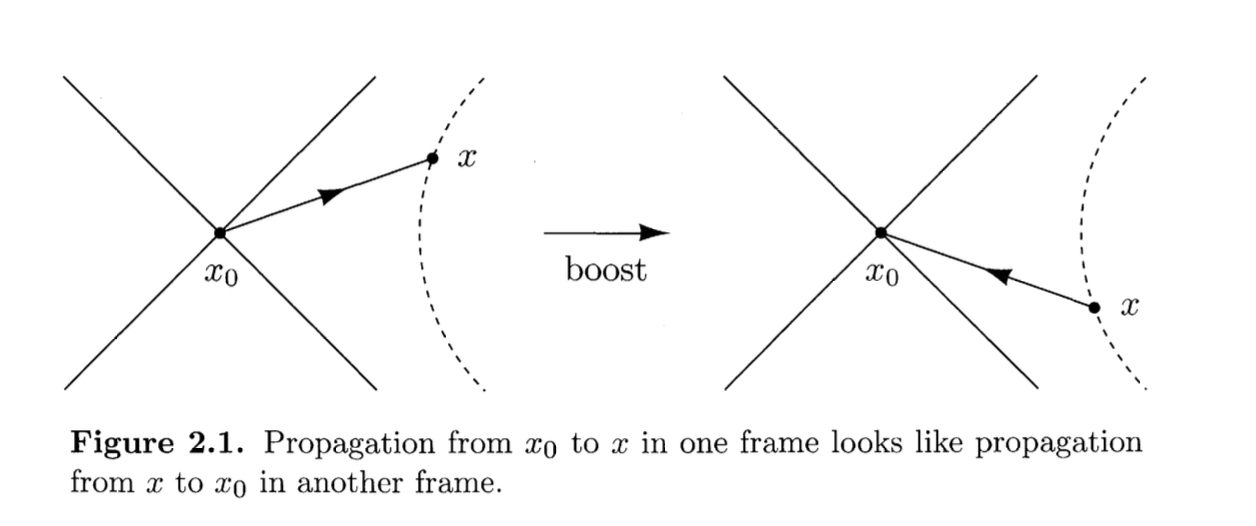
\includegraphics[width=1\textwidth]{./PsekinQFT_Sec2-1_fig/fig2-1.png}
\end{figure}

\noindent 場の量子論はこの因果律の問題を2.4節で述べるような見事な方法で解決する. 多粒子の場の理論では, space-like な距離に渡って伝播する粒子と, その逆方向に伝播する反粒子との差が付かない(Figre 2.1 参照). 点 $\boldsymbol{x}_0$ に於ける観測が点 $\boldsymbol{x}$ に於ける観測に影響を及ぼし得るかどうかを考えると, 粒子と反粒子の伝播確率振幅はちょうど打ち消し合い, 因果律は保たれる.
  
場の量子論では, 多粒子状態に限らず粒子数の異なる状態間の遷移を自然な形で扱える. また, 反粒子を導入することで因果律の問題を解決し, スピンと粒子の量子統計の関係を説明することができる. しかし最も重要なのは, 散乱断面積, 粒子の寿命といった無数の可観測量を計算するのに必要な道具が揃っていることである. 場の量子論が学ぶに値するのは, その予言がしばしば前例が無いほどの高い精密さでもって確かめられることにある.




\end{document}
